\documentclass[twocolumn]{article}
\usepackage[utf8]{inputenc}
\usepackage[margin=1in]{geometry}  % 调整页面边距
\usepackage{titling}               % 控制标题位置
\usepackage{booktabs}              % 表格宏包
\usepackage{amssymb}
\usepackage{ctex}                  % 中文支持包
\usepackage{authblk}			   % 多作者
\usepackage{graphicx}
\usepackage{ragged2e}           % 摘要两端对齐
% \usepackage{tabularx}			% 表格宽度
% \usepackage{xeCJK}
\setlength{\droptitle}{-3.0cm}     % 将标题上移3.0厘米

\title{v31 Medical Image Synthesis from CT to PET using Convolutional Neural Network}
\author[1] {Xiaoyu Deng}
\author[1,2] {Kouki Nagamune}
\author[1] {Hiroki Takada}
% \author[1] {Teacher Author}
% \author[1,3]{Third Author}
\affil[1]{University of Fukui, 3-9-1 Bunkyo, Fukui, 910-0019, Japan}
\affil[2]{University of Hyogo, 2167 Shosha, Himeji, Hyogo, 670-2280, Japan}
% \affil[3]{Research Institute, Company Z}
\date{ }

\begin{document}

\twocolumn[
	\maketitle

	\begin{center}
		\begin{abstract}
			\begin{justify}
				U-Net, a deep learning architecture, has gained widespread application in medical image processing due to its exceptional performance and efficient structural design. This architecture enhances traditional convolutional neural networks with its symmetric "U" shape, making it extensively utilized for applications such as image denoising, medical image registration, attenuation correction, lesion segmentation, and facial image restoration. This study leverages the U-Net architecture for cross-modality conversion from computed tomography to positron emission tomography images.
				Preliminary results demonstrate rapid performance improvements within the initial training epochs, achieving stability and high-quality reconstruction as training progresses. Despite observable fluctuations in performance metrics, which highlight the model's challenges in generalizing across the inherent variability of medical imaging datasets, the U-Net model exhibits robustness in image reconstruction. With further adjustments and optimizations, there is potential for enhanced performance in future applications, promising advances in the practical application of deep learning techniques in medical imaging.
			\end{justify}
		\end{abstract}
	\end{center}
	\vspace{0.5cm}  % 调整摘要与正文之间的间距
]

\section{Introduce}
U-Net 是一种最初为分割任务设计的深度学习架构,由于其出色的性能和高效的结构,在医学图像处理领域已变得非常流行。U-Net 的架构是对典型卷积神经网络(CNN)的改进,其特点是呈对称的“U”形,包括一个收缩路径(编码器)和一个扩张路径(解码器),也被称为编解码器结构。U-Net的一个关键特征是它使用了跳跃连接,将来自收缩路径的特征图连接到扩张路径中的相应层。这种设计使得网络能够在上采样过程中利用更精确的空间信息,这对于提高分割边界的准确性至关重要,尤其是在医学图像中结构描绘至关重要的地方。
增加UNet模型规模的方式有增加网络深度,增加特征图通道数,改进跳跃连接结构,融入Transformer等注意力模块等。这些改进可以提高模型的性能,但也会增加模型的复杂度和计算量且往往存在性能瓶颈,本研究使用多个简单的编解码器结构构建生成网络,验证多阶模型在医学图像生成任务中的性能。
本文的主要贡献在于使用多阶级联扩展框架,使用简单编解码器模型构建多个多阶级联模型进行CT到PET图像的转换任务,通过实验验证该扩展框架对于精度提升的有效性,并展示在每个阶段的模型中,U-Net模型在医学图像生成任务中的性能表现,以及在训练和测试过程中的多项指标变化情况。我们将对比不同阶段数的U-Net模型在CT到PET图像转换任务中的性能表现,在医学图像生成中的应用潜力。具体如下:
1.本文提出一种多阶级联扩展框架,在不改变单阶编解码器模型的情况下,使用多个简单的编解码器模型构建多个多阶级联模型进行肺部CT到PET图像的转换任务。
2.在基于公开数据上构建PETCT成对图像数据集上通过实验验证该扩展框架对于精度提升的有效性,并展示在每个阶段的模型中,U-Net模型在医学图像生成任务中的性能表现,以及在训练和测试过程中的多项指标变化情况。
3.我们将多个级联扩展模型转换后的图像与真实图像的视觉对比,探索级联扩展对生成图像的视觉质量的影响。

\section{Related Works}
自 Olaf 及其同事 \cite{navab_u-net_2015} 引入 U-Net 以来,由于其结构优势和在图像去噪、医学图像配准和衰减校正等应用中的出色性能,U-Net 已被广泛使用。它还应用于各种其他图像分割任务,包括病变分割,面部图像修复。
Armanious等人\cite{armanious_medgan_2020}提出了一种用于医学图像到图像的端到端框架,构建的GAN在PET-CT翻译,MR运动伪影校正和PET图像去噪等任务中验证了其性能。
Singh等人\cite{singh_automated_2023}提出了一种基于U-Net的自动化医学图像配准方法,通过GAN从未进行衰减矫正的PET图像生成伪CT图像,提高冠状动脉血管造影的配准效率和准确性。
Liu等人\cite{liu_deep_2018}开发了一种可从单个未经衰减校正的18F-FDG PET图像生成用于衰减校正的伪CT图像。
Du等人\cite{du_medical_2020}综述了六种基于U-Net结构的方法在医学图像分割中的应用,包括肺部结节分割、心脏分割、脑部分割等。
Zeng等人\cite{zeng_swin-casunet_2022}在面部图像修复任务中使用2阶级联的U-Net,展示了良好的性能,这表明多阶级联的U-Net在图像生成任务中具有潜在的优势。
Singh和Liu等人将通过微调模块的方式将模型应用在医学图像配准和衰减校正任务中,在专项领域内取得不错的效果。
Armanious和Zeng等人的工作使用了级联U-Net结构,但是并未探索多阶级联U-Net在医学图像生成任务中的性能。
本研究将使用多阶级联U-Net模型进行CT到PET图像的转换任务,并通过以下指标评估模型的性能。

结构相似性指数(SSIM)是一种复杂的指标,用于测量两幅图像之间的结构相似性。它考虑了图像的亮度、对比度和结构信息等因素。SSIM 值范围从 -1 到 1,其中 1 表示完全相似。该指标在医学图像分割中特别有用,因为它详细反映了图像的视觉和结构质量。

多尺度结构相似性指数(MS-SSIM)是 SSIM 的扩展,它跨多个尺度评估图像相似性,从而更全面地评估图像质量。这在处理分辨率差异很大的医学图像时特别有用。

峰值信噪比(PSNR)是另一种广泛用于测量图像重建质量的指标。它用于图像和视频压缩以及其他形式的信号处理等领域,通过比较原始图像和处理后图像之间的相似性来评估图像重建或压缩的质量。

平均绝对误差(MAE)是评估图像重建质量最常用的指标之一。它计算的是重建图像与原始图像之间像素强度差异的绝对值的平均值。MAE 值越低,图像重建中的误差越小,质量越高。与均方误差(MSE)相比,MAE 对异常值不敏感。在医学图像处理中,MAE 可以用于评估医学图像重建和分割算法的性能。在pytorch框架下,像素会被缩放到0到1之间,因此与MSE相比,MSE的值会更小,在一定程度上影响了轻视了像素误差的影响。因此本文选择MAE作为评估指标之一。


\section{Method}
Encoder-decoder architecture is designed symmetrically, with a contracting path to capture context and a symmetric expanding path that enables precise localization. This study aims to construct a standard U-Net, a convolutional neural network, to develop a cross-modality medical image converter from CT to PET images. The model will be optimized using a specific loss function suitable for this type of image conversion task.

本文提出的级联扩展框架所采用的网络结构主要包括编码器模块、解码器模块以及可视化模块。其中,编码器模块的作用是对输入图像进行特征提取,解码器模块则负责将编码器提取的特征图重建为输出图像,而可视化模块的功能则是进一步将输出图像转化为易于分析的可视化结果。单个编解码器模块的具体结构如图\ref{fig:Encoder_Decoder_Pair}所示。

% % TODO: \usepackage{graphicx} required
\begin{figure*}[t!]
	\centering
	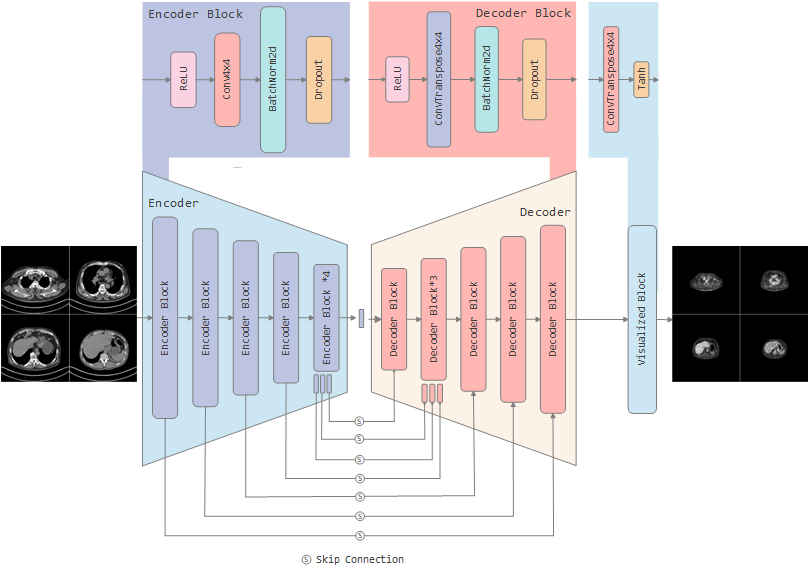
\includegraphics[width=1.0\linewidth]{u-net/lung/Encoder-Decoder-5layer-250406}
	\caption[architecture]{Schematic Diagram of Data Flow Within the Model. The PET image is shown on the left, and the CT image on the right. The blue modules correspond to the encoder architecture, while the orange modules represent the decoder architecture. The upper portion of the figure illustrates the fundamental structures of the encoder blocks, decoder blocks, and visualization blocks. The connections in the lower portion indicate the skip connections.}
	\label{fig:Encoder_Decoder_Pair}
\end{figure*}

\textbf{Encoder Block} The encoder follows the typical architecture of a convolutional network. It consists of repeated application of two $3\times3$ convolutions, each followed by a rectified linear unit (ReLU) and a $2\times2$ max pooling operation with stride 2 for downsampling. At each downsampling step, the number of feature channels is doubled. The convolution operation in U-Net can be described by the following equation:
\[
	I' = \sum_{i,j} (I * K)(i,j) + b
\]
where \(I\) represents the input image, \(K\) is the convolution kernel, \(b\) is the bias, and \(I'\) is the output feature map.

\textbf{Decoder Block} The decoder includes a series of upsampling and convolution operations. Each step in the expanding path includes an upsampling of the feature map followed by a $2\times2$ convolution that halves the number of feature channels, a concatenation with the correspondingly cropped feature map from the contracting path, and two $3\times3$ convolutions, each followed by a ReLU. Up sampling in the expanding path uses transposed convolutions to increase the size of the feature map:
\[
	U = K^T * I
\]
where \(K^T\) is the transposed convolution kernel and \(U\) is the upsampled output.

\textbf{Visual Block}(可视化模块)为一种变形的解码器模块,主要作用是将解码器模块生成的输出特征转换为可视化格式。其结构与标准解码器模块类似,但去除了跳跃连接,且所使用的非线性函数也有所不同。该模块的目的是将解码器输出进一步转化为便于分析的可视化图像。

\begin{table}[h]
	% \centering
	\caption{Encoder-decoder Setting Table}
	\label{tab:encoder_setting}
	\begin{tabular}{ccccc}
		\hline
		Block Name   & input & output & trans & dropout \\
		\hline
		Encoder 1    & 3     & 64     & -     & -       \\
		Encoder 2    & 64    & 128    & -     & -       \\
		Encoder 3    & 128   & 512    & -     & -       \\
		Encoder 4    & 256   & 512    & -     & -       \\
		Encoder 5    & 512   & 512    & -     & -       \\
		Encoder 6    & 512   & 512    & -     & -       \\
		Encoder 7    & 512   & 512    & -     & -       \\
		Encoder 8    & 512   & 512    & -     & -       \\
		Decoder 1    & 512   & 1024   & 512   & 0.5     \\
		Decoder 2    & 1024  & 1024   & 512   & 0.5     \\
		Decoder 3    & 1024  & 1024   & 512   & 0.5     \\
		Decoder 4    & 1024  & 1024   & 512   & -       \\
		Decoder 5    & 1024  & 512    & 256   & -       \\
		Decoder 6    & 512   & 256    & 128   & -       \\
		Decoder 7    & 256   & 128    & 64    & -       \\
		Visual Block & 128   & 3      & -     & -       \\
		\hline
	\end{tabular}
\end{table}

\subsection{级联扩展框架}
本文提出的级联扩展框架采用上述编解码器结构作为基本单元,通过将多个编解码器模块级联在一起,构建了一种多阶级联网络结构。每个编解码器的输出均作为下一级编解码器的输入,从而实现了逐级特征精炼的效果。该框架旨在通过级联多个编解码器,以提升模型的性能与准确性。这种结构设计使模型在各阶段能够捕获更丰富的特征信息,从而提高最终生成图像的质量。此外,理论上可采用不同阶段的输出计算损失函数,以进行分段优化,但本文未对此作进一步讨论。本文共构建了多个不同的级联编解码器模型,并引入了一个额外的包含密集连接和分段优化机制的模型,即DSGGAN。DSGGAN模型的结构与前述的级联扩展框架类似,但在各阶段输出处引入了密集连接与分段优化策略,从而更有效地捕捉不同阶段的特征信息,以进一步提升性能与精度。表\ref{tab:model_parameters}展示了不同模型的参数数量。

\begin{table}[h]
	\centering
	\caption{Parameters of Neural Networks.}
	\label{tab:model_parameters}
	\begin{tabular}{ccccc}
		\hline
		Architectures & Parameters \\
		\hline
		% Stage01       & 54.41      \\
		% Stage02       & 108.82     \\
		% DualSG      & 92.54      \\
		Stage03       & 163.24     \\
		Stage04       & 217.66     \\
		Stage05       & 272.07     \\
		Stage06       & 326.49     \\
		Stage07       & 380.90     \\
		Stage08       & 435.31     \\
		Stage09       & 489.73     \\
		Stage10       & 544.155    \\
		\hline
		\multicolumn{2}{p{201pt}}{The table depicts the Parameters of different generators. The quantity of parameters is expressed in millions.}
	\end{tabular}
\end{table}


\section{Experiments}
This study employs the encoder-decoer architecture for cross-modality medical image conversion tasks, specifically to construct a U-Net that inputs a CT image and converts it into a corresponding PET image. In this research, the lung PET or CT scan data were powered by the National Cancer Institute Cancer Imaging Program (CIP) \cite{li_large-scale_2020}.  The dataset encompasses 251,135 lung scan images from 355 subjects, primarily collected between 2009 and 2011, including each subject's gender, age, weight, smoking history, and cancer diagnosis classification. All scan data in the dataset are stored in DICOM format. This study processed these 251,135 scan data using the MicroDicom software on a Windows operating system. The subjects in the dataset are labeled according to the type of cancer: Type A for adenocarcinoma, Type B for small cell carcinoma, Type E for large cell carcinoma, and Type G for squamous cell carcinoma. Not all subjects' data include both PET and CT scans. 

因此,本研究选择了38位确诊为小细胞癌(Type B)患者的扫描数据,包括PET扫描、多种CT扫描及融合增强扫描图像。最终,我们获得了464对PET/CT图像数据,共计928张图像。本研究中,我们将数据分为训练集和测试集,其中训练集包含800张图像,测试集包含128张图像。数据集具体划分情况如表\ref{tab:dataset_partition_1}所示。

% 插入三线表
\begin{table}[h]
	\centering
	\caption{Dataset Partition of Experiment}
	\label{tab:dataset_partition_1}
	\begin{tabular}{cccc}
		\toprule
		Params count     & Test & Train & Total \\
		\midrule
		Lung PET/CT Pair & 64   & 400   & 464   \\
		Total Images     & 128  & 800   & 928   \\
		\bottomrule
	\end{tabular}
\end{table}

本实验采用标准的编解码器模型,以CT图像为输入,生成正电子发射断层扫描图像。优化过程中,我们采用了常用的均方误差和对抗损失来优化生成对抗网络。模型优化器选用Adam算法,学习率设为0.001,这种较低的学习率有助于模型在训练过程中逐渐逼近全局最优解。最优的实验结果如表\ref{tab:exps_result}所示。

\begin{table}[h]
	\centering
	\caption{Max SSIM,PSNR,MAE Results of Experiment}
	\label{tab:exps_result}
	\begin{tabular}{cccc}
		\toprule
		Stage Count & SSIM            & PSNR             & MAE             \\
		\midrule
		1 Stage     & 0.9149          & 27.7411          & 0.0119          \\
		2 Stages    & 0.9182          & 27.9950          & 0.0109          \\
		3 Stages    & 0.9060          & 27.6395          & 0.0127          \\
		4 Stages    & 0.9155          & 28.1969          & 0.0112          \\
		5 Stages    & 0.9104          & 26.6691          & 0.0130          \\
		6 Stages    & 0.9167          & 27.9794          & 0.0108          \\
		7 Stages    & \textbf{0.9255} & 27.1919          & 0.0116          \\
		8 Stages    & 0.9178          & 28.5503          & 0.0107          \\
		9 Stages    & 0.9093          & 28.7770          & 0.0109          \\
		10 Stages   & 0.9245          & \textbf{28.9168} & \textbf{0.0097} \\
		DSGGAN    & 0.9122          & 28.7630          & 0.0105          \\
		\bottomrule
	\end{tabular}
\end{table}

此外,实验针对每个模型记录了超过200个训练周期的数据,包括结构相似性指数、峰值信噪比和均方误差。每个训练周期结束后均进行了测试,记录的损失值及SSIM、PSNR和MAE指标的变化如各自对应图表所示。整体来看,各模型在训练集和测试集上均表现出良好的性能。且stage07模型和stage10模型在测试集上表现出更高的SSIM和PSNR值,表明其在图像重建任务中具有更好的性能。

\begin{figure}[h]
	\centering
	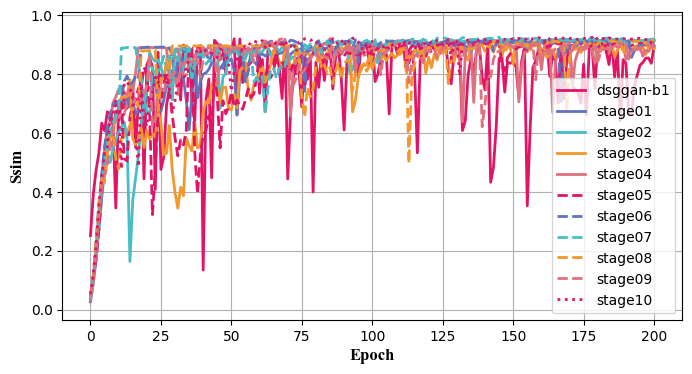
\includegraphics[width=1.0\linewidth]{u-net/lung/csv_stage01_10_dsg_lung_evalu_csv_img_2025_04_06_15_44_18/ssim_comparison}
	\caption[ssim]{SSIM Line Figure of All Epoch in Test Process}
	\label{fig:ssim}
\end{figure}

% 图 \ref{fig:ssim} 显示,在初始训练阶段(前 25 个轮次),所有模型测得的结构相似性指数 (SSIM) 值迅速增加,从接近零上升到 0.6 以上。这表明编解码器结构模型快速学习了 CT 和 PET 图像之间的映射关系,展现出显著的初始学习效果。在此快速增长之后,训练集和测试集上的 SSIM 值都趋于稳定,主要在 0.9 附近波动。这表明模型在持续的训练过程中保持了较高的图像重建质量。在整个训练集期间,dsggan模型的测试结果抖动较其他模型更大,这可能是由于模型将U-Net的跳跃连接改为了深度感知连接,过于重视高维的信息特征,但降低单组编解码器深度,导致模型的高维特征学习能力不足,造成了模型的抖动。整体来看,所有模型在训练集和测试集上的 SSIM 值都保持在较高水平,表明它们在 CT 到 PET 图像转换任务中表现良好。

如图\ref{fig:ssim}所示,在初始训练阶段(前25个周期),各模型的结构相似性指数(SSIM)迅速提升,由初始接近零快速上升至0.6以上,体现了编解码器结构在学习CT与PET图像间映射关系上的显著初始效果。随后,SSIM数值逐渐趋于稳定,在0.9附近波动,表明持续训练过程中各模型保持了较高的图像重建质量。其中,DSGGAN(dsggan)模型在测试集上表现出较大的波动,可能是由于该模型将U-Net的跳跃连接替换为深度感知连接,过于关注高维特征,反而限制了单个模块对高维信息的充分学习,导致模型表现波动较大。但总体而言,所有模型的SSIM指标均维持在较高水平,表明模型在CT至PET图像转换任务中效果良好。

\begin{figure}[h]
	\centering
	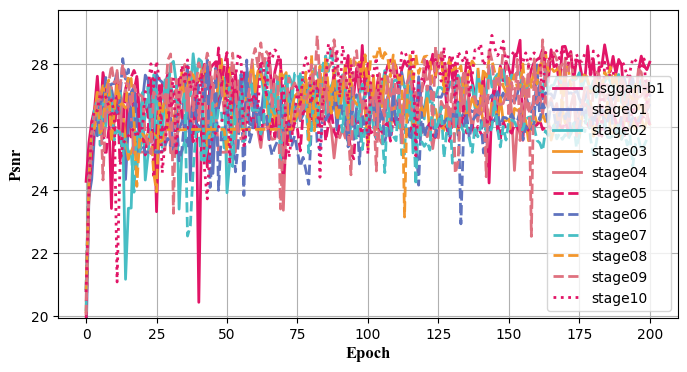
\includegraphics[width=1.0\linewidth]{u-net/lung/csv_stage01_10_dsg_lung_evalu_csv_img_2025_04_06_15_44_18/psnr_comparison}
	\caption[psnr]{PSNR Line Figure of All Epoch in Test Process}
	\label{fig:psnr}
\end{figure}

% 图 \ref{fig:psnr} 显示,与SSIM表现相似,峰值信噪比值在初始轮次中都迅速增加,这表明模型很快开始有效地从 CT 图像重建 PET 图像。最初的快速提升可能与模型参数的快速调整有关,显著提高了重建图像的质量。在最初的增长之后,在随后的过程中都出现了一些显著的波动。这些波动可能反映了模型在遇到数据中困难样本时或由于训练集规模较小,而导致的泛化性能较差从而产生的性能变化。尽管存在这些波动,所有模型的PSNR均保持在相近的水平,表明该系列模型能够完成重建 PET 图像任务。其中8阶模型和6阶模型5阶模型在训练的中后期出现过较大的波动,可能是由于模型在训练过程中对数据集的适应性不足,导致了性能的波动。

如图\ref{fig:psnr}所示,峰值信噪比(PSNR)的表现与SSIM类似,在训练初期快速提升,反映模型迅速开始有效地进行图像重建。初期快速提升的原因可能在于模型参数调整迅速。随后的训练过程中出现了明显的波动,尤其是8阶、6阶和5阶模型,这可能是模型在面对复杂数据或较小训练集规模时的泛化能力不足所致。尽管存在波动,所有模型的PSNR整体仍处于相近的水平,表明模型整体上能够有效完成图像重建任务。

\begin{figure}[h]
	\centering
	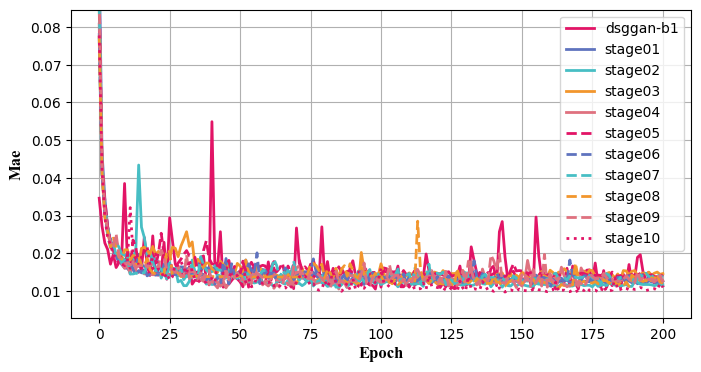
\includegraphics[width=1.0\linewidth]{u-net/lung/csv_stage01_10_dsg_lung_evalu_csv_img_2025_04_06_15_44_18/mae_comparison}
	\caption[mae]{MAE Line Figure of All Epoch in Train and Test Process}
	\label{fig:mae}
\end{figure}

% 从图 \ref{fig:mae} 可以观察到,在最初的几个轮次中,平均绝对误差 (MSE) 都从大约 0.08 的初始值迅速下降到 0.02 以下。这表明模型能够快速有效地适应从 CT 到 PET 的图像转换,学习速度很快。在快速下降之后,MAE 趋于稳定,尽管出现了几个明显的峰值,尤其是DSG-GAN模型,3阶模型。这些峰值可能反映了模型不同跳跃连接设计的影响。除了偶尔的峰值外,MAE 大部分时间都保持在较低水平,表明模型在整个过程中具有相对的稳定性。这表明模型在大多数情况下能够重建图像,且指标较好。
如图\ref{fig:mae}所示,平均绝对误差(MAE)在初期迅速从约0.08下降到0.02以下,表明模型快速有效地适应了CT至PET的图像转换任务。在随后的稳定过程中,出现了若干显著波动峰值,特别是DSGGAN与3阶模型,这可能是由不同跳跃连接结构设计导致的。尽管偶尔出现波动,MAE总体保持较低水平,体现了模型的稳定性与可靠性。


\begin{figure*}[t!]
	\centering
	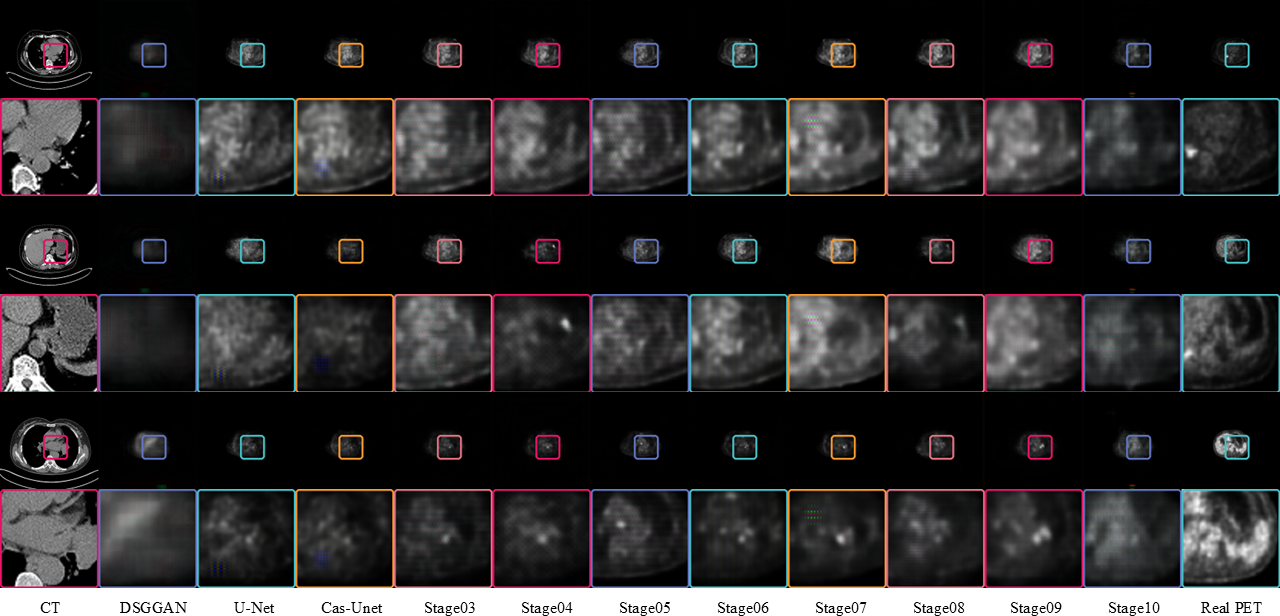
\includegraphics[width=1.0\linewidth]{u-net/lung/lung_compare_folder/lung_compare_13.png}
	% \caption[lung_compare]
	\caption[lung_compare]{The figure displayed here showcases PET images generated by various models, compared alongside real CT and PET images. The odd rows present the complete paired PET-CT images, while the even rows provide magnified views of specific regions within these pairs. Each model utilizes the CT image located at the extreme left as the input. The real PET images positioned at the extreme right serve as references for comparison. }
	\label{fig:lung_compare}
\end{figure*}
我们对所有模型生成的图像与真实图像进行了比较,如图\ref{fig:lung_compare}所示。尽管各模型在像素级指标表现较优,但视觉质量仍存在明显差异。尤其是stage03、stage04、stage05和stage07阶段产生了医学图像中不可接受的彩色棋盘格伪影,我们认为是由转置卷积上采样引起的图像失真。DualSGAN、U-Net及其他高级别模型虽未产生全局性伪影,但局部仍存在一些失真。此外,某些模型采用了过于追求模糊图像以优化指标的策略,这在视觉上并不理想。由此我们认为医学图像生成任务中,量化指标并不能完全代表图像的真实质量,需引入医学专家评估或先验知识指导训练。
% 我们将所有模型生成的图像与真实图像进行了对比,结果如图\ref{fig:lung_compare}所示。尽管所有模型生成的图像的各项像素级差异指标较好,但视觉上仍然存在较大差异。医学图像有其是PET图像,黑色区域占据图片较大面积,当模型学习到尽可能多的显示黑色及模糊的灰度图像即可获得较低较低,从而模型优化空间有限。在stage03,stage04,stage05,stage07中,均出现了彩色的棋盘格状图案,这种现象在医学图像中是不可接受的。我们认为这是在解码器阶段中,模型在上采样时使用转置卷积导致的图像失真和伪影。相反,DSGGAN,U-Net,Cas-Unet,stage06,stage08,stage09,stage10没有产生全局的彩色棋盘格图像,但在局部区域仍然存在一些伪影现象。而dsggan和stage10模型,均采用了生成尽可能模糊图像的策略,尽管在各项指标上较优,但其视觉表现直觉上并不匹配。尽管在没有见过样本中,多数模型生成的图像在视觉上仍然存在较大的差异,但也给了我们一些启示,即在医学图像Conversion任务中,生成图像的量化指标并不能完全反映图像的质量。我们认为,模型在训练过程中可能会学习到一些不必要的特征,从而导致生成图像的质量下降。因此,在医学图像Conversion任务中,除了量化指标外,还需要考虑生成图像的视觉质量,可能需要引入一些医学专家的意见来评估生成图像的质量,或者引入医学图像的先验知识来指导模型的训练。


\section{Conclusion}
本研究提出了一种级联扩展框架并进行了医学图像转换任务的实证研究。实验表明,该框架有效提高了模型的性能,并表现出较好的稳定性。然而,量化指标不能全面代表图像质量,因此未来研究中需兼顾视觉质量,引入专家评估或医学图像先验知识,以进一步提高医学图像转换的实用价值。

\section*{Acknowledage}
We would like to express our sincere gratitude to the National Cancer Institute Cancer Imaging Program for generously making their high-quality medical imaging dataset available and authorized for use on the Internet, providing indispensable resources for the smooth conduct of this research.

\bibliographystyle{unsrt}
\bibliography{unet_ref}

\end{document}
